\a{ש}\o{לו}\x{ם} \e{ל}\o{כ}\x{ל} \i{מי} \e{ש}\o{לו}\x{מ}\i{די}\x{ם} \i{ל}\x{ק}\o{רוא} \e{ב}\i{ע}\x{ב}\i{רי}\x{ת},

\a{ה}\x{כ}\a{ת}\x{ב} \a{ה}\i{ע}\x{ב}\i{רי} \u{הוא} \x{כ}\a{ת}\x{ב} \a{י}\e{פה}, \e{ו}\e{י}\x{ש} \o{לו} \o{שו}\a{ר}\i{שי}\x{ם} \a{ע}\i{תי}\i{קי}\x{ם}, \a{א}\a{ב}\x{ל} \x{כ}\e{ש}\o{לו}\x{מ}\i{די}\x{ם} \i{ל}\x{ק}\o{רוא} \o{בו} \i{מ}\a{י}\x{ד} \i{נ}\x{ת}\a{ק}\i{לי}\x{ם} \e{ב}\e{ב}\a{ע}\a{יה}: \x{כ}\o{מו} \e{ש}\a{א}\e{ת}\x{ם} \e{ב}\a{ט}\x{ח} \x{כ}\a{ב}\x{ר} \o{יו}\x{ד}\i{עי}\x{ם}, \u{הוא} \o{לא} \a{מ}\i{צי}\x{ג} \e{א}\x{ת} \o{כ}\x{ל} \a{ה}\e{מ}\x{י}\a{דע} \e{ש}\a{צ}\i{רי}\x{ך} \e{כ}\e{ד}\x{י} \i{ל}\x{ק}\o{רוא} \e{א}\x{ת} \a{ה}\i{מי}\i{לי}\x{ם} \e{ב}\a{ק}\u{לו}\x{ת}. \i{ב}\x{ש}\i{בי}\x{ל} \e{זה} \i{ב}\x{ד}\u{יו}\x{ק} \e{מ}\u{יו}\e{ע}\e{ד}\x{ת} \a{ה}\o{חו}\e{ב}\e{ר}\x{ת} \a{ה}\o{זא}\x{ת}: \e{ל}\a{ה}\x{ש}\i{לי}\x{ם} \e{א}\x{ת} \a{מה} \e{ש}\a{ח}\e{ס}\x{ר} \i{ב}\x{ש}\i{בי}\x{ל} \i{מי} \e{ש}\o{לו}\x{מ}\i{די}\x{ם} \i{ל}\x{ק}\o{רוא}, \e{ב}\o{כ}\x{ל} \i{גי}\x{ל}.

\a{ב}\a{ח}\x{ר}\i{תי} \a{כ}\a{מה} \e{ט}\x{ק}\x{ס}\i{טי}\x{ם} \e{ש}\a{א}\i{ני} \o{חו}\e{ש}\x{ב} \e{ש}\e{ה}\x{ם} \a{י}\i{פי}\x{ם} \u{ו}\e{מ}\a{ע}\x{נ}\e{יי}\i{ני}\x{ם}, \a{צ}\a{בע}\i{תי} \e{א}\x{ת} \a{ה}\o{או}\i{ת}\o{יו}\x{ת} \e{ו}\i{ה}\x{ש}\a{ל}\x{מ}\i{תי} \i{סי}\a{מ}\i{ני}\x{ם} \e{ש}\a{צ}\i{רי}\x{ך}.

\begin{framed}
	\a{ה}\o{או}\i{ת}\o{יו}\x{ת} \x{צ}\u{בו}\o{עו}\x{ת} \e{ל}\i{פי} \a{ה}\i{שי}\a{טה} \a{ה}\a{ב}\a{אה}~—
\begin{compactitem}
\item \e{צ}\a{בע} \a{כ}\e{זה}~\symbolglyph{\a{⬢}} \e{ב}\i{מי}\i{לי}\x{ם} \x{כ}\o{מו}: \a{ד}\x{ג}~(\symbolglyph{🐟}) או \a{צ}\x{ב}~(\symbolglyph{🐢})
\item \e{צ}\a{בע} \a{כ}\e{זה}~\symbolglyph{\e{⬢}} \e{ב}\i{מי}\i{לי}\x{ם} \x{כ}\o{מו}: \e{ע}\x{ז}~(\symbolglyph{🐐})
\item \e{צ}\a{בע} \a{כ}\e{זה}~\symbolglyph{\i{⬢}} \e{ב}\i{מי}\i{לי}\x{ם} \x{כ}\o{מו}: \i{פי}\x{ל}~(\symbolglyph{🐘})
\item \e{צ}\a{בע} \a{כ}\e{זה}~\symbolglyph{\o{⬢}} \e{ב}\i{מי}\i{לי}\x{ם} \x{כ}\o{מו}: \o{קו}\x{ף}~(\symbolglyph{🐒})
\item \e{צ}\a{בע} \a{כ}\e{זה}~\symbolglyph{\u{⬢}} \e{ב}\i{מי}\i{לי}\x{ם} \x{כ}\o{מו}: \u{סו}\x{ס}~(\symbolglyph{🐎})
\item \e{צ}\a{בע} \a{כ}\e{זה}~\symbolglyph{\x{⬢}} \x{כ}\e{ש}\e{א}\x{י}\x{ן} \x{ת}\u{נו}\a{עה}. (\x{כ}\o{מו} \e{ב}\o{סו}\x{ף} \a{ה}\e{ש}\o{מו}\x{ת} \a{ה}\e{א}\e{לה} \e{ש}\x{ל} \a{ה}\a{ח}\o{יו}\x{ת}).
\end{compactitem}

\a{א}\a{ח}\e{ר}\x{י} \a{ה}\a{ח}\o{יו}\x{ת}, \i{נ}\x{ת}\a{א}\e{מ}\x{ן} \x{ק}\a{צ}\x{ת} \i{ע}\x{ם} \x{כ}\e{ל}\x{י}־\e{ר}\e{כ}\x{ב}:\\
\i{ג׳י}\x{פ}~(\symbolglyph{🚙}),
\i{סי}\a{רה}~(\symbolglyph{⛵}),
\o{או}\o{טו}~/ \e{מ}\o{כו}\i{ני}\x{ת}~(\symbolglyph{🚗})
\x{ט}\a{ר}\x{ק}\o{טו}\x{ר}~(\symbolglyph{🚜}),
\a{מ}\o{טו}\x{ס}~(\symbolglyph{✈}),
\a{מ}\o{סו}\x{ק}~/ \e{ה}\i{לי}\o{קו}\x{פּ}\e{ט}\x{ר}~(\symbolglyph{🚁}),
\o{או}\o{טו}\u{בּו}\x{ס}~(\symbolglyph{🚌}),
\o{או}\i{ני}\a{יה}~(\symbolglyph{🚢}),
\a{ח}\x{ש}\a{מ}\i{לי}\x{ת}~(\symbolglyph{🚋}),
\a{כ}\a{בּ}\i{אי}\x{ת}~(\symbolglyph{🚒}),
\a{מ}\a{שׂ}\i{אי}\x{ת}~(\symbolglyph{🚚}),
\i{מי}\i{ני}\u{בּו}\x{ס}~(\symbolglyph{🚐}),
\a{ר}\e{כּ}\e{ב}\x{ל}~(\symbolglyph{🚡}),
\a{ר}\e{כּ}\e{ב}\x{ת}~(\symbolglyph{🚂}),
\o{או}\a{פ}\a{נ}\i{יי}\x{ם}~(\symbolglyph{🚲}).

\e{ו}\a{א}\a{ח}\e{ר}\x{י} \e{ש}\i{ה}\x{ת}\a{א}\a{מ}\u{נו}, \u{נו}\a{כ}\x{ל} \i{ל}\x{ק}\o{רוא} \i{מ}\x{ש}\a{פ}\x{ט} \e{ל}\u{דו}\x{ג}\a{מה}:\\
\a{ה}\i{כי} \e{כי}\x{ף} \i{ל}\x{ר}\a{כ}\x{ב} \a{ע}\x{ל} \o{או}\a{פ}\a{נ}\i{יי}\x{ם}~\symbolglyph{🚲}, \a{א}\a{ב}\x{ל} \a{א}\i{פי}\u{לו} \o{יו}\e{ת}\x{ר} \e{כי}\x{ף} \a{ל}\u{טו}\x{ס} \a{ל}\a{ח}\a{ל}\x{ל}~\symbolglyph{🚀}.

\i{סי}\a{מ}\i{ני}\x{ם} \o{נו}\a{ס}\i{פי}\x{ם}:
\begin{itemize}
	\item דגש (נקודה באמצע האות) מופיע באותיות ב׳, כ׳ ופ׳ כשהן לא בראש מילה והן נהגות כמו במילים „בובה” (), „” (), „פלפל” (). בראש מילה הן תמיד דגושות (במעט המילים שלא, יש קו קצר מעליהן, כמו במילים „\a{פֿ}\a{לא}\e{פ}\x{ל}” ו„\o{כֿו}\e{רי}\o{או}\x{ג}\a{ר}\x{פ}\a{יה}”).
	\item שין שׂמאלית סימנתי, והיא נהגית כמו סמ״ך.
	\item תנועת פתח גנובה עם חי״ת מסומנת בעיגול קטן, כך: \a{ת}\u{פו}\gnuva \x{ח}~(\symbolglyph{🍎}), \a{מ}\x{פ}\e{ת}\gnuva \x{ח}~(\symbolglyph{🔑}).
\end{itemize}

\end{framed}

%בחוברת הקטנה הזאת הזאת תוכלו למצוא טקסטים\footnote{„טקסט” זאת מילה משפה שנקראת לטינית, שפעם דיברו בה בהרבה איזורים בעולם, והמשמעות שלה היא „משהו שמישהו כתב/אמר”. היא מגיעה מהמילה „טקסטוס” (בלטינית: \LR{textus}), שאומרת „אריג, משהו ארוג” (אריגה היא שיטה ליצור בד מחוטים. הרבה שטיחים הם ארוגים). זה כאילו שהמילים והמחשבות הן חוטים, ומצרפים אותן ביחד (שלובות, קלועות, שזורות, ארוגות) כדי ליצור משהו חדש, אחר, שמורכב מהן. אם אתם מכירים את המילה „טקסטורה”, תשימו לב שהיא גם מגיעה מאותו המקור. בעברית קוראים לטקטסטורה גם „מרקם”, אבל רקמה היא בכלל מלאכת־יד אחרת בחוטים. אפשר לעשות בחוטים דברים יפיפיים, שלפעמים מפתיע שהם בסך־הכל חוטים מלופפים אחד בתוך השני (ולפעמים רק חוט אחד, כמו בסריגה!).
	
%	הדבר שאתם קוראים עכשיו נקרא „הערת־שוליים”, ולפעמים יש בהערות שוליים את הדברים הכי מעניינים בטקסט…} מעניינים ויפים לדעתי~— בעיקר שירים~— שאני חושב שיהיה לכם מעניין לקרוא.

%בעברית הכתב לא מוסר בפשטות את כל המידע שצריך כדי לדעת איך לקרוא את הטקסט. כן מסומנות תנועות, אבל לא תמיד ולא באופן מדוייק. במונחים של בלשנות זה נקרא אבג׳ד, וגם ערבית כותבים בכתב מסוג כזה (ולכן אפשר להשתמש בשיטה הזאת גם לערבית).

%כשלומדים לקרוא טקסטים לא מנוקדים, כמו שאתם עושים עכשיו, 

%השיטה היא פשוטה נורא: כל תנועה מסומנת בצבע אחר.


\a{ה}\o{חו}\e{ב}\e{ר}\x{ת} \a{ה}\o{זא}\x{ת} \o{חו}\x{פ}\i{שי}\x{ת}: \e{זה} \o{או}\e{מ}\x{ר} \e{ש}\e{א}\x{שׂ}\a{מ}\x{ח} \i{א}\x{ם} \a{ת}\a{ע}\i{תי}\u{קו} \o{או}\a{תה}, \a{ת}\a{ע}\u{שׂו} \a{בה} \i{שי}\u{נו}\i{יי}\x{ם} \e{ו}\a{ת}\i{פי}\u{צו} \o{או}\a{תה} \e{מ}\a{ח}\a{ד}\x{ש}. \e{א}\x{ת} \a{ה}\e{ט}\x{ק}\x{ס}\i{טי}\x{ם} \o{לא} \a{א}\i{ני} \i{חי}\a{בּ}\x{ר}\i{תי}, \a{א}\a{ב}\x{ל} \a{א}\e{ת}\x{ם} \u{מו}\x{ז}\a{מ}\i{ני}\x{ם} \a{ל}\a{ע}\o{שׂו}\x{ת} \a{מה} \e{ש}\a{א}\e{ת}\x{ם} \o{רו}\i{צי}\x{ם} \i{ע}\x{ם} \a{מה} \e{ש}\a{א}\i{ני} \a{ע}\i{שׂי}\i{תי}: \a{ה}\a{ר}\a{ע}\o{יו}\x{ן}, \a{ה}\i{בי}\u{צו}\a{ע}, \a{ה}\i{סי}\u{מו}\x{ן}. \e{א}\x{פ}\a{ש}\x{ר} \a{כ}\u{מו}\a{ב}\x{ן} \a{ג}\x{ם} \a{ל}\a{ק}\a{ח}\x{ת} \e{א}\x{ת} \a{ה}\a{ר}\a{ע}\o{יו}\x{ן} \e{ל}\e{ט}\x{ק}\x{ס}\i{טי}\x{ם} \a{א}\e{ח}\i{רי}\x{ם} \o{או} \e{ל}\a{שׂ}\o{פו}\x{ת} \a{א}\e{ח}\o{רו}\x{ת} (\e{ל}\u{דו}\x{ג}\a{מה}, \x{כ}\e{ש}\i{ת}\x{ל}\e{מ}\u{דו} \i{ל}\x{ק}\o{רוא} \e{ב}\a{ע}\a{ר}\i{בי}\x{ת}, \i{א}\x{ם} \a{א}\e{ת}\x{ם} \o{לא} \o{יו}\x{ד}\i{עי}\x{ם} \x{כ}\a{ב}\x{ר}). \a{ג}\x{ם} \o{כ}\x{ל} \a{ה}\o{תו}\x{כ}\o{נו}\x{ת} \e{ש}\i{ה}\x{ש}\a{ת}\a{מ}\x{ש}\i{תי} \a{ב}\e{ה}\x{ן} \e{כ}\e{ד}\x{י} \e{ל}\a{ה}\i{כי}\x{ן} \e{א}\x{ת} \a{ה}\o{חו}\e{ב}\e{ר}\x{ת} \e{ה}\x{ן} \o{חו}\x{פ}\i{ש}\o{יו}\x{ת}.

\u{תו}\x{כ}\u{לו} \i{ל}\x{מ}\o{צוא} \e{א}\x{ת} \a{ה}\o{חו}\e{ב}\e{ר}\x{ת}, \o{כו}\e{ל}\x{ל} \x{ק}\a{ב}\i{צי}\x{ם} \e{ש}\e{א}\x{פ}\a{ש}\x{ר} \e{ל}\a{ה}\i{צי}\x{ג} \e{ו}\a{ל}\a{ע}\o{רו}\x{ך} \a{ב}\a{מ}\x{ח}\e{ש}\x{ב}, \a{ב}\x{כּ}\o{תו}\e{ב}\x{ת} \a{ה}\o{זא}\x{ת}: \url{http://xpr.digitalwords.net/***}

\e{א}\x{שׂ}\a{מ}\x{ח} \e{ל}\a{ק}\e{בּ}\x{ל} \a{ה}\a{צ}\o{עו}\x{ת} \e{ל}\i{שי}\u{פּו}\x{ר}, \e{ט}\x{ק}\x{ס}\i{טי}\x{ם} \e{ל}\o{הו}\a{ס}\a{פה}, \i{תי}\u{קו}\i{ני}\x{ם}, \u{ו}\i{ב}\x{כ}\a{ל}\x{ל}, \e{א}\x{שׂ}\a{מ}\x{ח} \i{ל}\x{ש}\o{מו}\a{ע} \e{א}\x{ת} \a{מה} \e{ש}\e{י}\x{ש} \a{ל}\e{כ}\x{ם} \e{ל}\a{ה}\i{גי}\x{ד} (\e{ב}\o{כ}\x{ל} \e{ד}\e{ר}\x{ך}; \i{ב}\x{מ}\u{יו}\a{ח}\x{ד} \e{א}\x{שׂ}\a{מ}\x{ח} \e{ל}\a{ק}\e{בּ}\x{ל} \i{צ}\u{יו}\i{רי}\x{ם}, \a{ו}\a{א}\i{ני} \a{מ}\x{ב}\i{טי}\gnuva \x{ח} \i{ל}\x{ת}\o{לו}\x{ת} \o{או}\a{ת}\x{ם}…).

%\a{ג}\x{ם} \a{ה}\o{גו}\a{פ}\x{ן}\footnote{„\o{גו}\a{פ}\x{ן}” \e{זה} \a{ה}\u{צו}\a{רה} \a{ה}\e{מ}\u{סו}\e{יי}\e{מ}\x{ת} \e{ש}\x{ל} \a{ה}\o{או}\i{ת}\o{יו}\x{ת}. \o{כ}\x{ל} \o{או}\x{ת} \e{א}\x{פ}\a{ש}\x{ר} \i{ל}\x{כ}\o{תו}\x{ב} \e{ב}\i{ס}\x{ג}\o{נו}\o{נו}\x{ת} \o{שו}\i{ני}\x{ם}; \e{ב}\o{גו}\a{פ}\x{ן} \e{מ}\u{סו}\a{יי}\x{ם} \e{ל}\o{כ}\x{ל} \a{ה}\o{או}\i{ת}\o{יו}\x{ת} \i{ס}\x{ג}\o{נו}\x{ן} \o{דו}\e{מה}. \e{ל}\u{דו}\x{ג}\a{מה} (\i{שי}\u{מו} \e{ל}\x{ב} \a{ל}\u{צו}\a{רה} \a{ה}\o{שו}\a{נה} \e{ש}\x{ל} \a{ה}\o{או}\i{ת}\o{יו}\x{ת} \a{א}\e{ל}״\x{ף}, \a{ו}״\x{ו} \e{ו}\a{ת}״\x{ו} \e{ב}\o{כ}\x{ל} \o{גו}\a{פ}\x{ן}):
%	\begin{multicols}{3}
%		\noindent
%		{\fontspec{Guttman Hodes}\o{או}\x{ת} \a{ה}\a{ד}\a{סה}}\\
%		{\fontspec{Rutz_OE Regular Pro}\o{או}\x{ת} \a{ר}\x{ץ}}\\
%		{\fontspec{SBL Hebrew}\o{או}\x{ת} \x{ס}\x{ב}״\x{ל} \i{ע}\x{ב}\i{רי}\x{ת}}\\
%		{\fontspec{Guttman Hatzvi}\o{או}\x{ת} \a{ה}\x{צ}\i{בי}}\\
%		{\fontspec{Guttman Haim}\o{או}\x{ת} \a{ח}\i{יי}\x{ם}}\\
%		{\fontspec{Guttman Vilna}\o{או}\x{ת} \i{וי}\x{ל}\a{נא}}\\
%		{\fontspec{Frank Ruehl CLM}\o{או}\x{ת} \x{פֿ}\a{ר}\x{נ}\x{ק}־\i{רי}\x{ה}\x{ל}}\\
%		{\fontspec{David CLM}\o{או}\x{ת} \a{ד}\i{ו}\x{ד}}\\
%		{\fontspec{Narkisim}\o{או}\x{ת} \a{נ}\x{ר}\i{קי}\i{סי}\x{ם}}\\
%		{\fontspec{Guttman Keren}\o{או}\x{ת} \o{ק(ו)}\e{ר}\x{ן}}\\
%		~\\
%		\symbolglyph{☜}~{\fontspec{Alef}\o{או}\x{ת} \a{א}\e{ל}\x{ף}}
%	\end{multicols}
%} \e{ש}\e{מ}\a{ש}\e{מ}\x{ש} \a{ב}\o{חו}\e{ב}\e{ר}\x{ת} \u{הוא} \o{חו}\x{פ}\i{שי}. \o{קו}\x{ר}\i{אי}\x{ם} \o{לו} „\a{א}\e{ל}\x{ף}”, \e{ו}\e{ה}\i{כי}\u{נו} \o{או}\o{תו} \a{כ}\a{מה} \a{א}\a{נ}\i{שי}\x{ם} \o{טו}\i{בי}\x{ם} \e{ש}\a{ג}\x{ם} \e{ה}\x{ם} \i{י}\a{שׂ}\e{מ}\u{חו} \i{א}\x{ם} \i{י}\x{ש}\a{ת}\x{מ}\u{שו} \o{בו}, \a{י}\a{ע}\i{תי}\u{קו} \o{או}\o{תו} \e{ו}\e{י}\a{ש}\u{נו} \o{או}\o{תו}: \u{מו}\o{שו}\x{ן} \e{ז}\x{ר}־\a{א}\i{בי}\x{ב}, \i{מי}\a{כ}\x{ל} \a{ס}\a{ה}\x{ר}, \a{ד}\i{ני} \e{מ}\x{י}\a{ר}\x{ב} \e{ו}\i{ני}\x{ר} \e{יי}\i{ני}.\\
%***תו\x{כ}\u{לו} \i{ל}\x{ק}\o{רוא} \a{ע}\a{לי}\x{ו} \o{עו}\x{ד} \a{כא}\x{ן}: \url{http://alef.hagilda.com/}.

\e{מ}\a{ק}\e{ווה} \e{ש}\e{ת}\e{ה}\u{נו}~\symbolglyph{☺},\\
\u{יו}\a{דה},\\
\a{א}\a{בּא} \e{ש}\x{ל} \i{אי}\x{ל}\i{אי}\x{ל}, \e{ש}\a{ב}\a{ח}\a{רה} \e{א}\x{ת} \a{ה}\x{צ}\a{ב}\i{עי}\x{ם}

\LR{
a\mbox{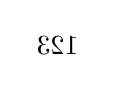
\begin{tikzpicture}\draw node [xscale=-1]{123};\end{tikzpicture}}b
}
